\begin{example}[From one coloring to three submitted states]
\label{ex:algorithm-submissions-20260918}
Continue \cref{ex:algorithm-banks-20260918}.  Set
$\DegreeCutoff=\ChunkCount=9$, so
$\ColorCount=8(\DegreeCutoff+1)=80$ and
$\ReadoutChunkSize=\lceil15/9\rceil=2$.
Fix one index $\tau\in[\ColoringCount]$ and suppose \AlgoBlockRef{draft}
draws the coloring
\[
 \ColorHash{\tau}{i}=
 \begin{cases}
 1,&i\in\{1,4\},\\
 2,&i\in\{10,13\},\\
 3,&i\in[15]\setminus\{1,4,10,13\}.
 \end{cases}
\]
These are three of the $80$ available colors, not a change to the
color-count parameter.  With
$\SourceColorValue=1$ and $\ReadoutColorValue=2$, \AlgoBlockRef{chunks}
applies \eqref{app:eq:color-class}--\eqref{app:eq:readout-chunks} to obtain
\[
 \ColorClass{\tau}{1}=\{1,4\},\qquad
 \ColorClass{\tau}{2}=\{10,13\},\qquad
 \mathcal C=\ReadoutChunk{\tau}{2}{1}=\{10,13\}.
\]
For this example only, write
$y^\kappa:=\ProbeState{\kappa}{\tau}{1}{\{10,13\}}$.
Because $G=\emptyset$, substituting the bank columns into
\eqref{app:eq:screen-probe-state} yields
\[
\begin{array}{c|cc|cc}
 &\multicolumn{2}{c|}{\text{src (source)}}
 &\multicolumn{2}{c}{\text{target (readout)}}\\
 \kappa&y^\kappa_1&y^\kappa_4&y^\kappa_{10}&y^\kappa_{13}\\ \hline
 1&a&b&\MASK&\MASK\\
 2&c&b&\MASK&\MASK\\
 \TailColumn&b&a&\MASK&\MASK
\end{array}
 \qquad
 y^\kappa_k=\DraftToken{k}=b
 \quad(k\in[15]\setminus\{1,4,10,13\}).
\]
These remaining positions are neither sources nor masked readouts.
Since $G=\emptyset$, they take the \emph{otherwise} branch of
\eqref{app:eq:screen-probe-state} and retain their draft values
$\DraftToken{k}$, which equal $b$ by \cref{ex:algorithm-banks-20260918}.
In \AlgoBlockRef{probes}, each of the three submissions returns both
$\OracleRow{y^\kappa}{10}$ and $\OracleRow{y^\kappa}{13}$.
Their role is to test dependence, not to commit the source tokens:
$G$ remains empty throughout.  In this particular example, column $1$
happens to agree with the draft at all unmasked positions; it is still
one of the three columns, not an extra baseline submission.
\Cref{fig:algorithm-submissions-20260918} shows these exact assignments.
\end{example}

\begin{figure}[tbp]
 \centering
 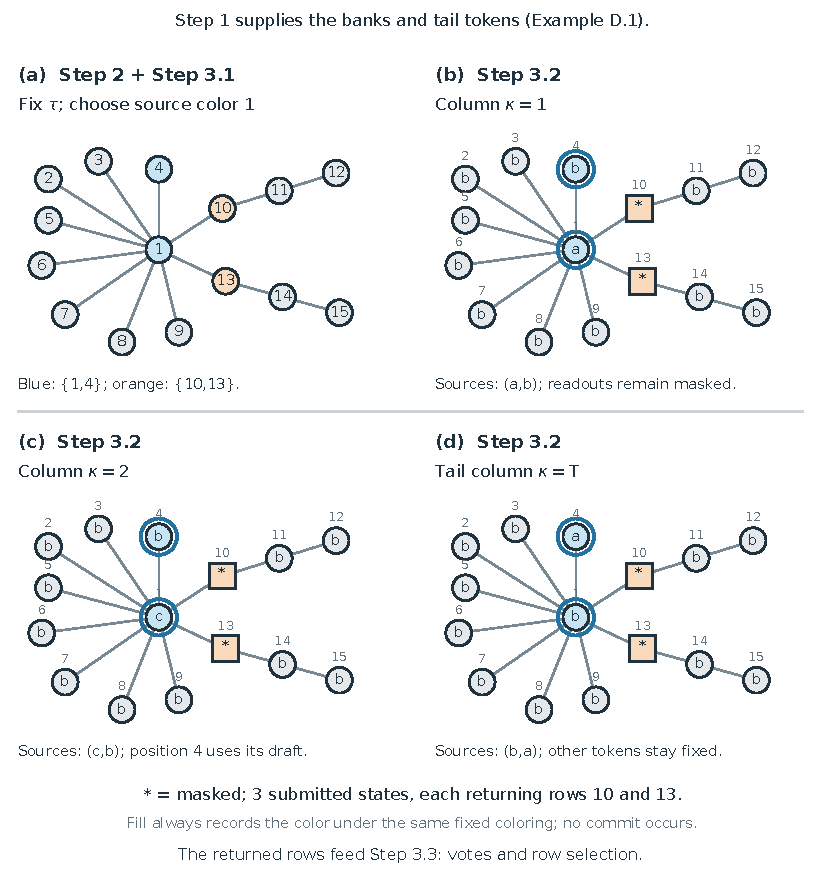
\includegraphics[width=\linewidth]{figures/algorithm_examples_2026-09-18/output/pdf/submissions_2026-09-18.pdf}
 \caption{The coloring and three submitted states of
 \cref{ex:algorithm-submissions-20260918}, labeled by the steps of
 Algorithms~\ref{app:alg:complete-sampler}--\ref{app:alg:packed-screen}.
 All $15$ positions are drawn
 separately at fixed locations. Fill denotes the color under $\tau$;
 square outlines mark masked readouts and double outlines mark sources.
 Small outer numbers are position indices, and inner symbols in
 (b)--(d) are submitted tokens. No vertex is committed by these probes.
 The hidden edges are shown only to explain the construction.}
 \label{fig:algorithm-submissions-20260918}
\end{figure}
